\documentclass{standalone}

\usepackage[euler-digits]{eulervm}

\usepackage{tikz}
\tikzset{every node/.style={circle,draw=none,minimum size=6mm,inner sep=0pt}}
\tikzset{t/.style={rectangle}}

\begin{document}
    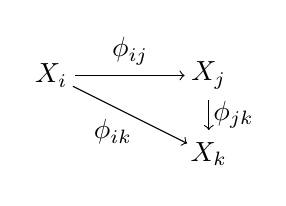
\begin{tikzpicture}[font=\sffamily]
      \node (i) at (0,0) {$X_i$};
      \node (j) at (2,0) {$X_j$};
      \node (k) at (2,-1) {$X_k$};
        \draw[->] (i) -- node[above] {$\phi_{ij}$}(j);
        \draw[->] (j) -- node[right] {$\phi_{jk}$} (k);
        \draw[->] (i) -- node[below left] {$\phi_{ik}$} (k);
    \end{tikzpicture}
\end{document}
